\documentclass{article}
\usepackage{amsmath}
\usepackage{relsize}
\usepackage{amssymb}
\usepackage{amsthm}
\usepackage[sc]{mathpazo}
\usepackage[T1]{fontenc}
\usepackage{geometry}
\geometry{verbose,tmargin=2cm,bmargin=2cm,lmargin=2.5cm,rmargin=2.5cm}
\setcounter{secnumdepth}{2}
\setcounter{tocdepth}{2}
\usepackage{url}
\usepackage{fancybox}
\usepackage{tikz}
\usepackage{bm}
%\usepackage[unicode=true,pdfusetitle,
% bookmarks=true,bookmarksnumbered=true,bookmarksopen=true,bookmarksopenlevel=2,
% breaklinks=false,pdfborder={0 0 1},backref=false,colorlinks=false]
%\hypersetup{
 %pdfstartview={XYZ null null 1}}
\usepackage{breakurl}
\usepackage{setspace}
\setlength{\textheight}{8.9in}
%\setbeamercolor{upcol}{fg=black,bg=gray}
%\setbeamercolor{lowcol}{fg=black,bg=gray!40}
\newcommand{\brown}[1]{\textcolor[rgb]{0.60,0.30,0.10}{#1}}
\newcommand{\sky}[1]{\textcolor[rgb]{0.00,0.38,0.62}{#1}}
\newcommand{\red}[1]{\textcolor[rgb]{0.90,0.00,0.10}{#1}}
\newcommand{\green}[1]{\textcolor[rgb]{0.00,0.70,0.30}{#1}}
\newcommand{\blue}[1]{\textcolor[rgb]{0.00,0.00,0.80}{#1}}
\newcommand{\purple}[1]{\textcolor[rgb]{0.50,0.00,0.50}{#1}}
\def\thickhrulefill{\leavevmode \leaders \hrule height 1ex \hfill \kern \z@}
\usepackage{Sweave}
\begin{document}
\input{lutfi_rdd-concordance}
%\SweaveOpts{concordance=TRUE}
%\SweaveOpts{concordance=TRUE}
%\SweaveOpts{concordance=TRUE}
%You need to change the options of Rstudio from Sweave to knitr to obtain 
% graphicsby doing: Rstudio->Preference->Sweave/pdf->change Sweave to Knitr
%Sweave2knitr("test1.Rww",output=)

\begin{center}
%  \includegraphics[width=1.75in]{ut1.png} 
\hrule height 1ex \vspace{2 pt} \hrule
\mbox{}\\
\mbox{}\\
{\large
\textbf{ECO395M  \hfill RDD Replication \hfill  Lutfi Sun}\\
\textbf{Causal Inference \hfill Assignment \hfill \today}}\\
\mbox{}
 \vspace{2 pt} \hrule \vspace{2 pt} \hrule height 1ex
\end{center}
% 
\vspace{0.5cm}





%%%%%%%%%%%%%%%%%%%%%%%%%%%%%%%%%%%%%%%%%%%%%%%%%%%%%%%%%%%%%%%%%%%%%%%%%%%%%%%%%%%%%%%%%%%%%%%%%%%%%%%%%
\section*{Part 1: Github Repo and Summary}
%%%%%%%%%%%%%%%%%%%%%%%%%%%%%%%%%%%%%%%%%%%%%%%%%%%%%%%%%%%%%%%%%%%%%%%%%%%%%%%%%%%%%%%%%%%%%%%%%%%%%%%%%

\textbf{1. Github Repository with Subdirectories and Data}
\begin{itemize}
  \item https://github.com/lutfisun/RDD.git
\end{itemize}
\textbf{2. Summarize Hansen AER}
\newline
\newline
What is his research question? 
\begin{itemize}
  \item Do the legal thresholds of 0.08 and 0.15 in Blood Alcohol Content (BAC) level effectively reduce drunk driving?
\end{itemize}
What data does he use?  
\begin{itemize}
  \item Hansen uses Washington State Administrative Records. The original data includes 512,964 Driving Under Influence (DUI) stops from 1995 to 2011.
  \item He utilizes a subset of this data (146,626) from 1999 to 2007 on stops of individuals over 21.
  \item He focuses on post 1999 because thresholds changed in 1999 and on those above 21 because cutoffs are different for those below legal drinking age.
\end{itemize}
What is his research design, or “identification strategy”?  
\begin{itemize}
  \item His identification strategy is a Local Liner Regression Discontinuity Design with Rectangular Kernel. He wants to show there is a significant difference in behavior between those slightly above either threshold and those slightly below.
  \item Identification Assumption 1: It is by random chance for someone to be barely below or barely above the threshold.
  \begin{itemize}
    \item To support this claim, Hansen plots distribution of BAC levels (Figure 1). The distribution shows no sign of endogenous sorting, which implies people near the cutoffs do not self sort (or at least, there is no evidence that they do).
  \end{itemize}
  \item Identification Assumption 2: Police do not endogenously test people around the thresholds.
  \begin{itemize}
    \item To support this claim, table 2 shows predetermined characteristics such as race or age don't have much to do with being above or below the BAC thresholds.
  \end{itemize}

\end{itemize}
What are his conclusions?
\begin{itemize}
  \item The 0.08 threshold leads to a 2\% point decline in recidivism for the next four years. The 0.15 aggrevated DUI cutoff corresponds to an additional percentage point decline.
  \item The reduction in repeated drunk driving can be explained via deterrence channel. Those above the threshold are more likely to receive a harsher punishment: higher fines, longer jail time, etc.
  \item This study presents evidence that reducing the BAC threshold or internalizing the costs of drunk driving by higher fines can be effective policies and curb DUI incidents.
\end{itemize}

%%%%%%%%%%%%%%%%%%%%%%%%%%%%%%%%%%%%%%%%%%%%%%%%%%%%%%%%%%%%%%%%%%%%%%%%%%%%%%%%%%%%%%%%%%%%%%%%%%%%%%%%%
\newpage
\section*{Part 2: Reproducing Hansen's Results}
%%%%%%%%%%%%%%%%%%%%%%%%%%%%%%%%%%%%%%%%%%%%%%%%%%%%%%%%%%%%%%%%%%%%%%%%%%%%%%%%%%%%%%%%%%%%%%%%%%%%%%%%%

\input{tmpout/t-setup}

{\tiny \setstretch{0.01} .}\\
\textbf{3. Create a dummy equaling 1 if bac1>= 0.08 and 0 otherwise in your do file or R file.}
\begin{Schunk}
\begin{Sinput}
 hansen <- read_dta("../data/hansen_dwi.dta")
 hansen$dui08 <- ifelse(hansen$bac1 >= 0.08, 1, 0)
\end{Sinput}
\end{Schunk}

\textbf{4. Do you find evidence for sorting on the running variable?}

\begin{centering}
\input{tmpout/t-mcgraph1}
\includegraphics{tmpout/t-mcgraph1}
\end{centering}

\begin{centering}
\begin{Schunk}
\begin{Sinput}
 density <- rddensity(hansen$bac1, c = 0.08, p=2, h=0.01)
 rdplotdensity(density, 
               hansen$bac1,
               plotN = 10,
               histBreaks= seq(from = 0, to =0.3 , by = 0.0039),
               histFillShade = 0.8)
\end{Sinput}
\end{Schunk}

\includegraphics{tmpout/t-mcgraph2}
\end{centering}

\begin{itemize}
  \item The McCrary density test with default settings in DCdensity function gives a p-value of 7.7e-07$<0.01$. This indicates that there is strong evidence of self sorting in the data.
  \item For bandwidth equals 0.02 on the two sides of the cutoff, the model does not catch any sign of manipulation. Meanwhile, as we go towards a lower bandwidth (say 0.01), there seems to be a difference between the two sides. The right side of 0.08 starts with a big jump in density in comparison to the left side.
  \item A similar jump is also visible in the Histogram of BAC levels when we have a large number of bins. This contradicts with what Hansen shows in his Figure 1 on page 1587.
  \item It is important to note, however, that we are only looking at a single BAC test. In reality, these tests are conducted twice and the lower value is considered to be the true one. So, a more realistic approach would be to look at signs of manipulation in the minimum of the two (bac1 and bac2) instead of in one of them as we are doing here for the sake of simplicity.
\end{itemize}

\begin{centering}
\begin{Schunk}
\begin{Sinput}
 hist(hansen$bac1,
      main="Histogram for BAC Levels Recorded in DUI Stops", 
      xlab="BAC",
      breaks = 40000)
 abline(v = 0.08, col= 'red')
\end{Sinput}
\end{Schunk}

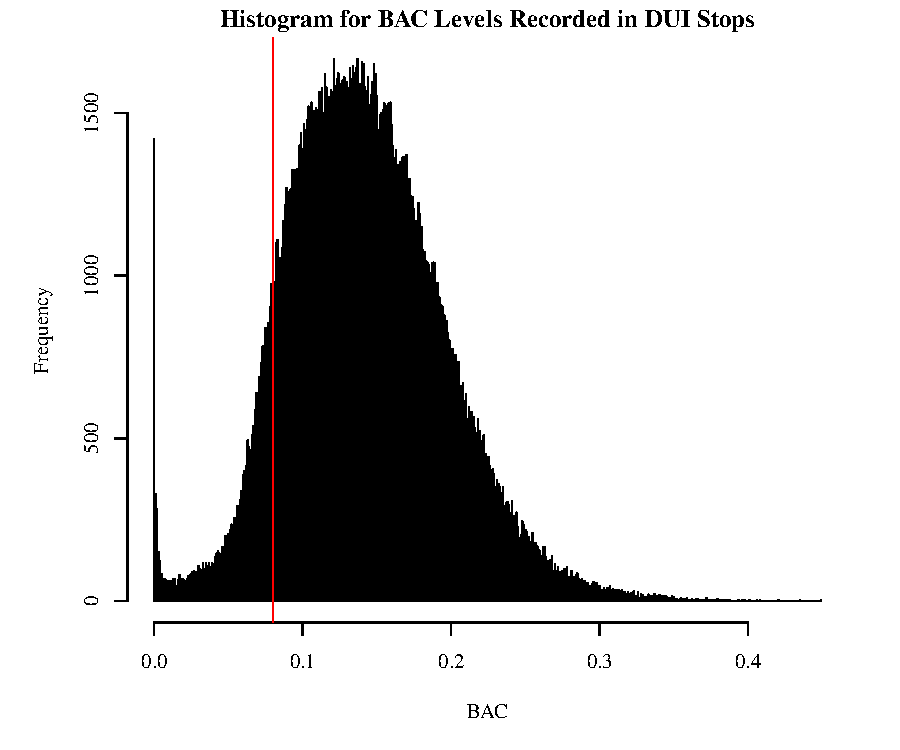
\includegraphics{tmpout/t-hist_bac}
\end{centering}

{\tiny \setstretch{0.01} .}\\
\textbf{5. Are the covariates balanced at the cutoff?}
\begin{Schunk}
\begin{Sinput}
 hansen$bac_centered <- hansen$bac1 - 0.08 
 # the slopes would not change whether we center or not (the intercept would)
 # so i decided not to center. it'll make it easier for predictions and graphs 
 weights <- rdd::kernelwts(hansen$bac1, 
                           center = 0.08, 
                           bw = .05, 
                           kernel = "rectangular")
 lm_1 <- lm_robust(male ~  bac1 + dui08 + bac1*dui08, data = hansen, weights = weights)
 lm_2 <- lm_robust(white ~ bac1 + dui08 + bac1*dui08, data = hansen, weights = weights)
 lm_3 <- lm_robust(aged ~ bac1 + dui08 + bac1*dui08, data = hansen, weights = weights)
 lm_4 <- lm_robust(acc ~ bac1 + dui08 + bac1*dui08, data = hansen, weights = weights)
 texreg::screenreg(list(lm_1, lm_2, lm_3, lm_4), 
                   custom.model.names = c("Male", "White", "Age", "Accident"))
\end{Sinput}
\begin{Soutput}
===========================================================================
             Male           White          Age               Accident      
---------------------------------------------------------------------------
(Intercept)       0.80 *         0.84 *        39.45 *            0.17 *   
             [ 0.77; 0.83]  [ 0.81; 0.87]  [ 38.51;  40.40]  [ 0.15;  0.20]
bac1             -0.21           0.08         -69.16 *           -1.10 *   
             [-0.68; 0.26]  [-0.34; 0.50]  [-83.32; -55.01]  [-1.46; -0.73]
dui08            -0.02           0.00          -6.22 *           -0.15 *   
             [-0.06; 0.02]  [-0.03; 0.04]  [ -7.37;  -5.08]  [-0.18; -0.12]
bac1:dui08        0.31           0.02          76.05 *            1.89 *   
             [-0.21; 0.82]  [-0.44; 0.47]  [ 60.67;  91.42]  [ 1.49;  2.29]
---------------------------------------------------------------------------
R^2               0.00           0.00           0.00              0.00     
Adj. R^2          0.00           0.00           0.00              0.00     
Num. obs.    214558         214558         214558            214558        
RMSE              0.00           0.00           0.02              0.00     
===========================================================================
* Null hypothesis value outside the confidence interval.
\end{Soutput}
\end{Schunk}


\begin{Schunk}
\begin{Sinput}
 lm_01 <-  lm(male ~ bac1 + dui08 + bac1*dui08, data = hansen, weights = weights)
 lm_02 <-  lm(white ~ bac1 + dui08 + bac1*dui08, data = hansen, weights = weights)
 lm_03 <-  lm(acc ~ bac1 + dui08 + bac1*dui08, data = hansen, weights = weights)
 lm_04 <-  lm(aged ~ bac1 + dui08 + bac1*dui08, data = hansen, weights = weights)
 stargazer(lm_01, lm_02, lm_03, lm_04)
\end{Sinput}
\end{Schunk}


% Date and time: Tue, Mar 02, 2021 - 20:55:06
\begin{table}[!htbp] \centering 
  \caption{The Effect of Exceeding The 0.08 Threshold on Covariates} 
  \label{} 
\begin{tabular}{@{\extracolsep{5pt}}lcccc} 
\\[-1.8ex]\hline 
\hline \\[-1.8ex] 
 & \multicolumn{4}{c}{\textit{Dependent variable:}} \\ 
\cline{2-5} 
\\[-1.8ex] & male & white & aged & acc \\ 
\\[-1.8ex] & (1) & (2) & (3) & (4)\\ 
\hline \\[-1.8ex] 
 bac1 & $-$0.210 & 0.079 & $-$69.164$^{***}$ & $-$1.096$^{***}$ \\ 
  & (0.240) & (0.210) & (6.844) & (0.178) \\ 
  & & & & \\ 
 dui08 & $-$0.018 & 0.004 & $-$6.224$^{***}$ & $-$0.154$^{***}$ \\ 
  & (0.020) & (0.017) & (0.564) & (0.015) \\ 
  & & & & \\ 
 bac1:dui08 & 0.307 & 0.016 & 76.049$^{***}$ & 1.888$^{***}$ \\ 
  & (0.263) & (0.230) & (7.508) & (0.196) \\ 
  & & & & \\ 
 Constant & 0.801$^{***}$ & 0.840$^{***}$ & 39.453$^{***}$ & 0.171$^{***}$ \\ 
  & (0.016) & (0.014) & (0.455) & (0.012) \\ 
  & & & & \\ 
\hline \\[-1.8ex] 
Observations & 214,558 & 214,558 & 214,558 & 214,558 \\ 
R$^{2}$ & 0.0001 & 0.0001 & 0.002 & 0.002 \\ 
Adjusted R$^{2}$ & 0.00002 & 0.0001 & 0.002 & 0.001 \\ 
Residual Std. Error (df = 89963) & 0.001 & 0.001 & 0.039 & 0.001 \\ 
F Statistic (df = 3; 89963) & 1.519 & 3.897$^{***}$ & 70.505$^{***}$ & 45.207$^{***}$ \\ 
\hline 
\hline \\[-1.8ex] 
\textit{Note:}  & \multicolumn{4}{r}{$^{*}$p$<$0.1; $^{**}$p$<$0.05; $^{***}$p$<$0.01} \\ 
\end{tabular} 
\end{table}

\begin{itemize}
  \item In Table 1 above, we are interested in the coefficient for the interaction term between bac1 and dui08 variables.
  \item We see that the covariates Age and Accident are not balanced around the cutoff. We observe more incidents with accidents right after the 0.08 threshold. This suggests that being considered a DUI incident is endogenous to whether the stop involves an accident (or whether the person is older) for BAC values near 0.08 (as we are using a local linear regression).
\end{itemize}
{\tiny \setstretch{0.01} .}\\
\textbf{6. Recreate Figure 2 panel A-D. Fit both linear and quadratic with confidence intervals.}

\begin{Schunk}
\begin{Sinput}
 grid_bac <- hansen %>%
   mutate(bacbin = cut(bac1, breaks = 
                         seq(from = -0.01, to = 4.01, by = 0.01))) %>%
   group_by(bacbin) %>%
   summarize(bac1 = mean(bac1, na.rm = TRUE),
             mean_male = mean(male, na.rm = TRUE),
             mean_white = mean(white, na.rm = TRUE),
             mean_age = mean(aged, na.rm = TRUE),
             mean_acc = mean(acc, na.rm = TRUE))
 grid_bac$dui08 <- ifelse(grid_bac$bac1 >= 0.08, 1, 0)
 pred_male <- predict(lm_01, grid_bac, interval="prediction")
 pred_white <- predict(lm_02, grid_bac, interval="prediction")
 pred_age <- predict(lm_03, grid_bac, interval="prediction")
 pred_acc <- predict(lm_04, grid_bac, interval="prediction")
 
\end{Sinput}
\end{Schunk}


\begin{Schunk}
\begin{Sinput}
 par(mfrow=c(2,2))
 plot(grid_bac$bac1, grid_bac$mean_male,
      main = "Panel A. Male - Linear",
      xlab = "bac level", ylab = "percentage male")
 polygon(c(rev(grid_bac$bac1), grid_bac$bac1), 
         c(rev(pred_male[ ,3]), pred_male[ ,2]), 
         col=adjustcolor("grey80",alpha.f=0.5), border = NA)
 lines(grid_bac$bac1, pred_male[,1], col=4)
 lines(grid_bac$bac1, pred_male[,2], lty = 'dashed', col=2)
 lines(grid_bac$bac1, pred_male[,3], lty = 'dashed', col=2)
 abline(v = 0.08, col= 1)
 plot(grid_bac$bac1, grid_bac$mean_white,
      main = "Panel B. White - Linear",
      xlab = "bac level", ylab = "percentage white")
 polygon(c(rev(grid_bac$bac1), grid_bac$bac1), 
         c(rev(pred_white[ ,3]), pred_white[ ,2]), 
         col=adjustcolor("grey80",alpha.f=0.5), border = NA)
 lines(grid_bac$bac1, pred_white[,1], col=4)
 lines(grid_bac$bac1, pred_white[,2], lty = 'dashed', col=2)
 lines(grid_bac$bac1, pred_white[,3], lty = 'dashed', col=2)
 abline(v = 0.08, col= 1)
 plot(grid_bac$bac1, grid_bac$mean_age,
      main = "Panel C. Age - Linear",
      xlab = "bac level", ylab = "average age")
 polygon(c(rev(grid_bac$bac1), grid_bac$bac1), 
         c(rev(pred_age[ ,3]), pred_age[ ,2]), 
         col=adjustcolor("grey80",alpha.f=0.5), border = NA)
 lines(grid_bac$bac1, pred_age[,1], col=4)
 lines(grid_bac$bac1, pred_age[,2], lty = 'dashed', col=2)
 lines(grid_bac$bac1, pred_age[,3], lty = 'dashed', col=2)
 abline(v = 0.08, col= 1)
 plot(grid_bac$bac1, grid_bac$mean_acc,
      main = "Panel D. Accident - Linear",
      xlab = "bac level", ylab = "percantage with accident")
 polygon(c(rev(grid_bac$bac1), grid_bac$bac1), 
         c(rev(pred_acc[ ,3]), pred_acc[ ,2]), 
         col=adjustcolor("grey80",alpha.f=0.5), border = NA)
 lines(grid_bac$bac1, pred_acc[,1], col=4)
 lines(grid_bac$bac1, pred_acc[,2], lty = 'dashed', col=2)
 lines(grid_bac$bac1, pred_acc[,3], lty = 'dashed', col=2)
 abline(v = 0.08, col= 1)
 
\end{Sinput}
\end{Schunk}

\includegraphics{tmpout/t-panel_a-d}

\begin{itemize}
  \item Comparing bac below and above 0.08, we see a change in slope especially for age and accident variables.
  \item Note: the confidence intervals for panel C and D are visible when I run the graphs on R but not visible when I compile pdf using sweave for some reason :/
\end{itemize}

\begin{Schunk}
\begin{Sinput}
 par(mfrow=c(2,2))
 plot(grid_bac$bac1, grid_bac$mean_male,
      main = "Panel A. Male - Local Quad",
      xlab = "bac level", ylab = "percantage with accident")
 lines(locfit(hansen$male ~ 
                lp(hansen$bac1, nn=0, h=0.05, deg=2)), col=5)
 abline(v = 0.08, col= 1)
 plot(grid_bac$bac1, grid_bac$mean_white,
      main = "Panel B. White - Local Quad",
      xlab = "bac level", ylab = "percantage with accident")
 lines(locfit(hansen$white ~ 
                lp(hansen$bac1, nn=0, h=0.05, deg=2)), col=5)
 abline(v = 0.08, col= 1)
 plot(grid_bac$bac1, grid_bac$mean_age,
      main = "Panel C. Age - Local Quad",
      xlab = "bac level", ylab = "percantage with accident")
 lines(locfit(hansen$aged ~ 
                lp(hansen$bac1, nn=0, h=0.05, deg=2)), col=5)
 abline(v = 0.08, col= 1)
 plot(grid_bac$bac1, grid_bac$mean_acc,
      main = "Panel D. Accident - Local Quad",
      xlab = "bac level", ylab = "percantage with accident")
 lines(locfit(hansen$acc ~ 
                lp(hansen$bac1, nn=0, h=0.05, deg=2)), col=5)
 abline(v = 0.08, col= 1)
 
\end{Sinput}
\end{Schunk}

\includegraphics{tmpout/t-quad_panel_a-d}

{\tiny \setstretch{0.01} .}\\
\textbf{7. Estimate equation (1) with recidivism (recid) as the outcome: Table 3 column 1}
\newline
\begin{itemize}
  \item yo
\end{itemize}
{\tiny \setstretch{0.01} .}\\
\textbf{8. Recreate the top panel of Figure 3.}
\newline
\begin{itemize}
  \item yo
\end{itemize}
{\tiny \setstretch{0.01} .}\\
\textbf{9. Discuss what you learned from this exercise.}
\newline
\begin{itemize}
  \item yo
\end{itemize}
What was the hypothesis you tested and what did you find?
\begin{itemize}
  \item yo
\end{itemize}
How confident are you in Hansen’s original conclusion? Why/why not?
\begin{itemize}
  \item yo
\end{itemize}
%%%%%%%%%%%%%%%%%%%%%%%%%%%%%%%%%%%%%%%%%%%%%%%%%%%%%%%%%%%%%%%%%%%%%%%%%%%%%%%%%%%%%%%%%%%%%%%%%%%%%%%%%

\end{document}












